% 

\documentclass[11pt]{article}
\usepackage[utf8]{inputenc}
\usepackage[T1]{fontenc}
% https://tex.stackexchange.com/questions/167402/how-to-set-font-size-at-exactly-11-pt
\usepackage[scaled=1.00375]{uarial}  % Arial is required (https://www.dfg.de/formulare/54_01/54_01_de.pdf, p.3)
\usepackage{amsmath,amssymb,amsfonts}
\usepackage{algorithmic, cite}
\usepackage{graphicx}
\usepackage{textcomp}
\usepackage{xcolor}
\usepackage{diagbox}
\usepackage{eurosym}
\usepackage{booktabs}
\usepackage{multicol}
\usepackage{multirow}
\newcommand{\todo}[1]{\textcolor{red}{#1}}
\usepackage{geometry}

\usepackage[subtle]{savetrees}

% make sure that reference sections are numerated
% as sections
% https://tex.stackexchange.com/questions/88890/how-to-get-the-references-section-to-be-numbered-as-if-it-were-created-via-sect
\usepackage[numbib]{tocbibind}

% additional bibliography for project-related publications
\usepackage[labeled, resetlabels]{multibib}
\newcites{pro}{Project-Related Publications}
\bibliographystylepro{IEEEtran}
\bibliographystyle{IEEEtran}

% according to https://www.sascha-frank.com/latex-font-size.html, if the main font size is 11, \footnotesize corresponds to 9, which is as tiny as we are allowed (https://www.dfg.de/formulare/54_01/54_01_en.pdf, p. 3)
\let\oldbibliography\thebibliography
\renewcommand{\thebibliography}[1]{%
  \footnotesize
  \oldbibliography{#1}%
  \setlength{\itemsep}{-1pt}%
}

\geometry{
  left=2cm,
  right=2cm,
  top=2cm,
  bottom=2cm,
  bindingoffset=5mm
}
\usepackage{setspace}


\usepackage{hyperref} % Should come last
\hypersetup{
   colorlinks,
   menucolor=black,
%   linkcolor=black,
%   citecolor=black,
   linkcolor=blue,
   citecolor=blue,
   urlcolor=blue
}
%Define references for Work Packages
\newcommand{\wpdef}[2]{\hypertarget{sec:W#1}{\paragraph*{(W#1) #2}\label{sec:W#1}}}
\newcommand{\WP}[1]{\hyperlink{sec:W#1}{W#1}}
\newcommand{\wpref}[2]{\hyperlink{sec:W#1}{#2}}

\newcommand{\objdef}[2]{\paragraph*{(#1) #2}\hypertarget{obj:#1}}
\newcommand{\objref}[1]{\hyperlink{obj:#1}{(#1)}}

\usepackage{enumitem}
\newenvironment{packed_enumerate}{
\begin{enumerate}[topsep=0pt, partopsep=0pt]
  \setlength{\itemsep}{0pt}
  \setlength{\parskip}{0pt}
  \setlength{\parsep}{0pt}
}{\end{enumerate}}

% =======================================================================
\begin{document}
\begin{center}

{\large \textbf{Proposal for the Research Grants Programme of the
German Research Foundation (Deutsche Forschungsgemeinschaft, DFG)}}
    
\end{center}

\vspace{.5cm}


% =======================================================================
\section*{General Information}
% =======================================================================

\begin{tabular}[t]{ll} 
Name: & \textbf{Prof. Dr.-Ing. Sebastian Stober} \\
Position: &  Full Professor\\
Date of Birth: &  10.12.1980\\
Nationality: &  German\\
Institution: &  Otto von Guericke University Magdeburg (OVGU)\\
Address (work): & Faculty of Computer Science, IKS-AiLab, Universitätsplatz 2, 39106 Magdeburg\\
Phone: & +49 391 67-58314\\
Fax: &  +49 391 67-42018\\
E-mail: & stober@ovgu.de\\
Address (private): & Eisenbahnstr. 33, 14542 Werder (Havel)\\
Phone: & +49 1520 4793669\\
\multicolumn{2}{l}{Reference number of a previous DFG grant proposal: STO 1145/2-1}\\
& \\
Name: & \textbf{Dr.-Ing. Jakob Abe{\ss}er} \\
Position: & Senior Scientist \\
Date of Birth: & 03.05.1983 \\
Nationality: & German \\
Institution: & Fraunhofer Institute for Digital Media Technology (IDMT) \\
Address (work): & Ehrenbergstraße 31, 98693 Ilmenau\\
Phone: & +49 3677 467288\\
Fax: & +49 3677 467467 \\
E-mail: & jakob.abesser@idmt.fraunhofer.de\\
Address (private): & Annemarie-Becker-Straße 16, 99092 Erfurt\\
Phone: & +49 176 61104420\\
\multicolumn{2}{l}{Reference number of a previous DFG grant proposal: AB 675/2-1}\\


\end{tabular}

\vspace{1cm}

\noindent \textbf{Topic}: \underline{So}und \underline{Re}cognition 
%in acoustic scenes 
via \underline{L}istening, \underline{U}nderstanding, and \underline{A}daptation (SoReLUA) \\
\textbf{Subject Area}: Computer Science, Artificial Intelligence, Image and Language Processing \\
\textbf{Keywords}: Acoustic Scene Understanding, Audio Event Detection, Machine Learning \\ % Machine Listening?
\textbf{Duration (in months)}: 36 (New Proposal) \\
%


% =======================================================================
\section*{Project Description}
% =======================================================================

% =======================================================================
\section{Starting Point}
% =======================================================================

% =======================================================================
\subsection{State of the Art and Preliminary Work}
% =======================================================================

% =======================================================================
%\subsubsection*{State of the Art} % (2.5 pages)}
% =======================================================================

%Legen Sie bei Neuanträgen den Stand der Forschung bitte knapp und präzise in seiner unmittelbaren Beziehung zum konkreten Vorhaben dar. In dieser Darstellung sollte deutlich werden, wo Sie Ihre eigenen Arbeiten eingeordnet sehen und zu welchen der anstehenden Fragen Sie einen eigenen, neuen und weiterführenden Beitrag leisten wollen. Der aktuelle Stand der eigenen Vorarbeiten ist zu benennen. Die Darstellung muss ohne Hinzuziehen weiterer Literatur verständlich sein.

% TODO in jedem Paragraf: 
% 1) wichtigste bestehende ansätze auflisten und erklären
% 2) eigene Forschung einordnen (in the SoReLUA project, we want to build upon ... )

% =======================================================================
\subsubsection{Sound Event Detection}
% =======================================================================

Machine listening algorithms combine methods from audio signal processing and machine learning with the goal of mimicking the human's ability to perceive and analyze complex acoustic scenes \cite{Virtanen:2018:SoundSceneBook:BOOK }.
Each acoustic scene commonly includes multiple sound sources, which emit different acoustic events (sounds) over time.
%Machine listening algorithms find application in various scenarios such as context-aware hearing aids, acoustic condition monitoring in industrial settings, biodiversity monitoring \cite{Lostanlen:2019:EventDetection:PLOS}, and smart cities.
% task definition ASC / AED
The two main directions of research in machine listening are acoustic scene classification (ASC) \cite{Barchiesi:2015:ASC:SPM}\citepro{Abesser:2020:ASC:AS} and sound event detection (SED).
While the goal of the former task is to summarize an entire recording using semantic labels such as ``traffic'' and ``office'', the latter task deals with the detection and classification of distinct sound events like ``sheep'' or ``door knock''. In the following section, we will focus on methods for sound event detection as they allow for the characterization of complex acoustic scenes based on audible sound events. 
%In this section, we will first discuss the main challenges of AED.
Due to the large number of recent publications, we will focus on the most relevant research trends in deep-learning based SED published over the last three years.
We refer the reader to two extensive overview articles \cite{Xia:2019:EventDetection:CSSR, Dang:2017:SurveyAED:ICOT} for a detailed summary of earlier SED approaches.

\paragraph{Challenges}
Computational methods for SED face several challenges in the analysis of complex acoustic scenes.
\begin{packed_enumerate}
    \item Environmental sounds exhibit a large range of different timbre characteristics such as short transients, noise, and harmonic signal components.
% Sound events of interest range from nature sounds like bird calls, rustling leaves, and rain drops, over machine-made sounds such as motor engines, braking noises, or chainsaws, to human-made sounds like voice, laughter, or screams. 
They can be characterized as structured or unstructured, stationary or non-stationary, repetitive or without any predictable nature.
    \item The duration of acoustic events cover a large range from very short (gun shots, door knocks, or shouts) to very long and almost stationary (running machines or climate sounds such as wind or rain). Since most SED methods analyze fixed-size audio segments, the classification of acoustic events is complicated, if the sound duration exceeds the segment size.
    \item The temporal boundaries (start and end times) of environmental sounds are often ill-defined, which complicates their precise annotation as well as the evaluation of SED algorithms. 
%For example, the loudness of passing vehicles like cars or trains gradually increase in the beginning and continuously fade into the background noise level at the end.
    \item Sound events appear either in the foreground or background depending on the relative position of the corresponding sound sources within an acoustic scene.
If multiple sounds appear simultaneously, the phase-dependent overlap often results in novel and unheard mixture sounds.
\end{packed_enumerate}

%Two possible solutions to unravel such mixtures from multi-channel audio recordings are source separation\footnote{\url{http://dcase.community/challenge2020/task-sound-event-detection-and-separation-in-domestic-environments}}, which aims at isolating individual sound sources, and sound localization\footnote{\url{http://dcase.community/challenge2019/task-sound-event-localization-and-detection}}, which aims at estimating the spatial position of sound sources from multi-channel audio recordings. 
%In this project, we will neither investigate source separation nor spatial sound localization since most machine listening datasets that we aim to exploit only provide monaural audio recordings. 
%The main reason for that is that single-channel recording setups are less expensive and easier to distribute in real-life machine listening application scenarios.

\paragraph{Network Architectures}

State-of-the-art SED algorithms apply deep neural networks for feature learning and classification.
The most common neural network architectures are convolutional neural networks (CNN) and convolutional recurrent neural networks (CRNN). 
Both architectures include a convolutional front-end, where multiple convolutional layers are trained to learn sound-specific features.
As input to the network, either fixed two-dimensional signal transformations such as mel spectrograms \cite{Hou:2019:SoundEvent:ICASSP}, or raw one-dimensional audio samples are used  \cite{Cakir:2018:EndtoEndAED:IJCNN} following an end-to-end learning approach. 
A specialized signal processing method for SED is per-channel energy normalization (PCEN) \cite{Lostanlen:2018:PCEN:SPL}, which combines dynamic range compression to reduce the loudness variance of foreground sounds and adaptive gain control to suppress stationary background noise.
As a back-end, CNN models use fully-connected layers for sound classification whereas CRNN models apply recurrent layers such as Gated Recurrent Units (GRU) or Long Short-Term Memory (LSTM) layers to model the temporal progression of the features extracted by the front-end.
% In the following, we will highlight several challenges of existing neural network based SED algorithms, which we aim to address in this project.

\paragraph{Transfer Learning \& Attention}

% DATASET IMBALANCE & SIZE - TRANSFER LEARNING / EMBEDDINGS
Machine listening datasets are often imbalanced since some sound classes naturally occur less frequent than others. Furthermore, annotating audio recordings is an extensive process which limits the amount of data for each event class, especially when new classes need to be detected or existing ones should be refined. 
Representation learning has shown to be a promising approach to train SED algorithms based on small and unbalanced datasets. Here, neural networks are pre-trained for a general classification task using a large dataset and then fine-tuned using a smaller task-specific datasets \cite{Arora2017}.
Given for instance a CNN model, one or multiple convolutional layers can be fixed after being pre-trained on a source task and the remaining layers can be fine-tuned on a new target task. The approach of using
intermediate feature representations (embeddings) of the final CNN layers as signal representation was successfully applied in the fields of SED/ASC. Commonly used embeddings are the OpenL3 embeddings \cite{Cramer2019:openl3},  the embeddings proposed by Kumar et al. \cite{Kumar2018:embedding}, VGGish embeddings \cite{Hershey:2017:CNN:ICASSP}, PANN (Pretrained Audio Neural Networks) embeddings \cite{Kong2019:PANN:ARXIV}, as well as the COALA (Co-Aligned Autoencoders) embeddings \cite{Favory:2020:COALA:ARXIV}, which are learnt by aligning latent representations of audio signals and the associated tags. Embeddings such as OpenL3 demonstrated their potential in various audio domains such as industrial sound analysis or MIR \cite{Grollmisch2020:embeddings}. % ATTENTION
Improvements in SED systems were achieved by introducing self-attention mechanisms. As an example, gated CNNs \cite{Xu:2018:WeaklyLabeledEventDetection:ICASSP} applied additional multiplicative gates to convolutional layers to better focus on particular feature map regions. 
%A similar gating mechanism is used in the recurrent layer to improve the temporal localization of sound events.
% DILATED CONVOLUTIONS / RECEPTIVE FIELD
The receptive field size of convolutional networks significantly influences the performance and robustness of machine listening algorithms towards unseen data \cite{Koutini:2019:ReceptiveField:DCASE}.
It can be increased by using dilated convolutions \cite{Li:2020:DilatedCRNN:ARXIV} or by replacing the convolutional and recurrent layers in a CRNN model by depth-wise separable and dilated convolutional layers \cite{Drossos:2020:SED:ARXIV}. % As a side effect, the number of model parameters and the training time can be reduced significantly. 
%Contrary, Koutini et al. report that models like ResNets tend to overfit for ASC tasks, if their receptive fields are not carefully constraint \cite{Koutini:2019:ReceptiveField:DCASE}.


% =======================================================================
\subsubsection{Acoustic Anomaly Detection}\label{sec:AD}
% =======================================================================

The task of anomaly detection (AD) is to detect deviations from a ``normal'' system state or behaviour.
%by analyzing different data modalities such as time series data, audio, or video recordings.
%AD is relevant for many application scenarios ranging from medical heart monitoring \cite{Ahrens2019}, intrusion detection \cite{Zieger:2009:Surveillance:AVSS}, to
%predictive maintenance of industrial facilities \citepro{Grollmisch:2019:ISA:EUSIPCO}. 
From the machine learning perspective, the biggest challenge of AD is that in most cases, only training examples from the normal system state are available while recordings from the anomalous state are often hard to acquire.
Given for instance an acoustic machine condition monitoring task in an industrial production site, it is too expensive or even impossible to simulate all possible machine faults.
Furthermore, anomalies often manifest in subtle sound variations while louder but irrelevant background noises must be ignored at the same time.

Traditionally, AD was approached by modeling the normal state data distribution using for instance Gaussian Mixture Models (GMM) or Support Vector Machines (SVM) in combination with outlier detection strategies in order to detect anomalies.
% Techniques such as Gaussian Mixture Models (GMM) or Support Vector Machines (SVM) are often used for distribution modeling. 
%before the class likelihood of a novel data instance can indicate whether its an anomaly or not.
A second approach for AD is to apply time-series modeling techniques such as auto-regressive models, Kalman filters, and Hidden Markov Models (HMM) to generate predictions on future data samples. 
An anomaly score can be computed from the deviation between a measured quantity at a certain point in time and its prediction based on previous observations.
%Nowadays, predictions are derived using non-linear methods such as recurrent and convolutional neural networks.
A third approach for AD is to apply autoencoders \cite{hinton2006autoencoders,vincent2010stacked,baldi2012autoencoders} which first compress an input signal into a low-dimensional representation using the encoder component and then attempt to reconstruct the original signal using the decoder component. Various techniques are used to guide the training process in such a way that the learned internal representation models only the essential features of the input, while all variance of the data, which is insignificant for modeling, is filtered out. If such an autoencoder is trained on examples from the normal state distribution, the reconstruction error for anomalous signals will likely be higher, and can therefore be used for AD. Popular autoencoder variants are fully-connected, convolutional, and include variational autoencoders.
A recent approach for AD in non-stationary machine sounds aims at interpolating a spectrogram frame from its previous and subsequent frames \cite{Hayashi2020}. 
An in-depth review of deep learning based AD techniques is provided in \cite{Chalapathy:2019:AD:ARXIV}.





% Instead of performing AD on raw measurement data, low-dimensional signal representations are processed during the time-series analysis.
%For instance, Lin et al.  use a Variational Autoencoder (VAE) to first extract low-dimensional embeddings from short time series segments. Then, they use an LSTM network to predict the embedding of the next time frame and derive the anomaly score from the deviation between the measured and predicted embedding. 
% Another way to reduce the data dimensionality is to initially perform a subsampling \cite{Kawaguchi:2017:SubsamplingAD:2017, Cherdo:2020:UnsupervisedAD:ICASSP}.

% ? https://arxiv.org/abs/1906.02845 out-of-distribution modeling

% % =======================================================================
% \paragraph{Audio Segmentation}
% % =======================================================================

% - analogy to music information retrieval\\
% - brief summary 
% - traditional approaches \\
% - representation learning (unsupervised learning using triplet loss \cite{McCallum:2019:Segmentation:ICASSP}\\
% - pre-processing step in semi-supervised annotation approaches for candidate segment selection \cite{Zhao2020} \\


% =======================================================================
\subsubsection{Machine Listening Datasets}
% =======================================================================

%As a general challenge in research fields such as computer vision, natural language processing, and machine listening, large datasets are required to capture and learn the natural variability within the data.
In this section, we want to highlight several publicly available sound event detection datasets with importance to the SoReLUA project. 
The two largest datasets for environmental sound analysis are the AudioSet dataset \cite{Gemmeke:2017:Audioset:ICASSP} (2.1 million audio clips, 527 sound classes) and the FSD50k dataset \cite{Fonseca:2020:FSD50K:ARXIV} (51,197 audio clips, 200 sound classes).
An example for a ``medium-scale'' SED dataset is the  ``Dataset for Environmental Sound Classification (ESC-50)''\footnote{\url{https://github.com/karolpiczak/ESC-50}} (2000 audio clips, 50 sound classes), which was used as evaluation set in over 50 scientific publications.
%includes include 2000 ten second recordings from 50 sound classes from the categories animal sounds, nature sounds, human-made sounds, interior (domestic), as well as exterior sounds. The dataset was used as evaluation set in over 50 scientific publications.
%In all runs of the annual ``DCASE'' evaluation campaign (Challenge on Detection and Classification of Acoustic Scenes and Events) since 2016,
%several tasks related to acoustic event detection in domestic and outdoor recordings were proposed with their unique datasets. 
%\footnote{For instance: TUT Sound events 2016, Development dataset \url{https://zenodo.org/record/45759}}. 
% As one example, 
The TUT Rare Sound Events dataset\footnote{\url{http://dcase.community/challenge2017/task-rare-sound-event-detection}} (3000 audio clips, 3 sound classes) 
and the CHIME-HOME dataset\footnote{\url{https://archive.org/details/chime-home}} 
are suitable datasets for evaluating SED algorithms in domestic environments.
% mention that most of these dataset come from Tampere University
SED datasets for analyzing urban sounds are the MAVD dataset\footnote{\url{https://zenodo.org/record/3338727}} and the Urban Sound Dataset\footnote{\url{https://urbansounddataset.weebly.com/}}. Several audio datasets with a focus on industrial sound analysis were published recently by Fraunhofer IDMT \citepro{Grollmisch:2019:ISA:EUSIPCO}
including audio recordings of different machine types and conditions\footnote{\url{https://www.idmt.fraunhofer.de/en/publications/datasets.html}}.
The ToyADMOS dataset \cite{Koizumi2019d} and MIMII dataset \cite{Purohit2019a} are recently published benchmark datasets for acoustic anomaly detection in industrial settings. 
As an example for natural sounds, the Xeno-Canto Bird Recordings Extended dataset\footnote{\url{https://www.kaggle.com/rohanrao/xeno-canto-bird-recordings-extended-a-m}} provides bird vocalization recordings from various species.

% =======================================================================
\subsubsection{Data Augmentation \& Domain Adaptation}
% =======================================================================

In order to mitigate the problem of limited dataset sizes, data augmentation techniques allow to create variations of existing data instances.
Commonly used transformations include audio signal processing such as pitch shifting, time stretching, or adding different types of noise  \cite{Salamon:2017:ASC:SPL, Xu:2018:ASCMobileNet:ISM}.
SpecAugment and Random Erasing are two techniques, which apply temporal warping and different kinds of noise masking to spectrograms \cite{Park:2019:SpecAugment:INTERSPEECH,Zhong:2017:RandomErasing:ARXIV}.
The most often used technique is mixup data augmentation \cite{Zhang:2018:Mixup:ICLR} in which two data instances as well as their targets are blended in a defined mixing ratio.
% As shown in \cite{Johnson2020:isa_normalization}, a random combination of data augmentation techniques like Mixup, SpecAugment, and pitch shifting/time stretching increases the robustness of SED algorithms in industrial settings to different recording conditions.%This allows for instance to simulate more complex acoustic scenes by mixing isolated sounds into the foreground and background. A combination of data augmentation and adaptive data normalization has been shown to improve SED systems for industrial sound analysis \cite{Johnson2020:isa_normalization}.


The performance of SED algorithms is often impaired by a distribution mismatch between training and test datasets (covariate shift) \citepro{Abesser:2020:ASC:AS}.
During the deployment in real-life scenarios, changes in the used recording devices as well as environmental influences can change the acoustic properties of recorded sound.
As a solution, the robustness of SED algorithms can be improved by domain adaptation (DA) methods. Here, these algorithms are adapted from the initial source domain (training) data to a novel target domain~\cite{Gharib:2018:DomainAdaptationASC:DCASE}.
As two examples, a supervised DA method using a factorized hierarchical variational autoencoder is proposed in \cite{Mun:2019:DomainMismatch:ICASSP}.
In case no annotations are available, unsupervised strategies can be followed to unify the source and target domain distributions \cite{Gharib:2018:DomainAdaptationASC:DCASE, Drossos:2019:DomainAdaptation:WASPAA}.

%In total, they cover over 30000 recordings of different operating states of vehicles such as toy cars, conveyors, and trains as well as machines such as valves, pumps, and fans.

%As an example of a dataset for environmental monitoring, we want to mention the BirdVox-70k\footnote{\url{https://zenodo.org/record/1226427#.Wt46UWaZO8o}}, which provides annotated field recordings for bird migration monitoring.

% - discuss weakly vs. strong labels \\
% - summarize most important datasets in table (size, classes, ...)\\

% =======================================================================
%\paragraph{Data Augmentation}
% =======================================================================


% =======================================================================
\subsubsection{Data Synthesis}
% =======================================================================
Additional training data for neural networks can be created using synthesis algorithms such as Generative Adversarial Networks (GAN) \cite{Goodfellow:2014:GAN:NIPS}, which imitate new examples by observing existing data instances (adversarial training). As an alternative to GAN-based algorithms, the SampleRNN model synthesizes audio signals on a sample-by-sample level. This model has been shown to be capable of creating realistic environmental sounds \cite{Kong:2019:SceneGeneration:ICASSP}.
Data synthesis methods either synthesize new examples as audio signals \cite{Mun:2017:ASC:ICASSP, Chen:2019:ASC:DCASE} or as intermediate embedding vectors \cite{Mun:2017:GANASC:DCASE}.  
%Autoencoders \cite{hinton2006autoencoders,vincent2010stacked,baldi2012autoencoders} transfer their input data by means of an encoder into an internal representation, from which the input data must be reconstructed by a decoder. 
%Encoders and decoders are trainable neural networks, which in principle can take any (task-related) form. 
%Various techniques are used to guide the training process in such a way that the learned internal representation models only the essential features of the input, while all variance of the data, which is insignificant for modeling, is filtered out. 
Generative models \cite{salakhutdinov2015learning} are trained with the learning task to generate data that are as similar as possible to real training data. 
The learned data generation process can provide information about the decisive factors underlying the data.

The ideas of autoencoders (cf.~\ref{sec:AD}) and generative models are combined in Variational Autoencoders (VAEs) \cite{kingma2013vae,rezende2014vae}. 
Here the decoder becomes a generative model which generates likely data for a given characteristic description (the internal representation). 
This technique also makes it possible to consider uncertainties and noise in the observation process. 
Furthermore, the characteristics learned by VAEs are often better interpretable than in other deep generative models.
There is a large number of variants of VAEs, which are particularly suitable for discrete feature spaces \cite{vandenoord2017vqvae,razavi2019vqvae2} or sequential modeling \cite{gregor2018tdvae}, and thus, represent suitable candidates for solutions in the SoReLUA project.

A new development that promises nothing less than a paradigm shift in VAEs and that is one essential component of the solution proposed here is Differential Digital Signal Processing (DDSP) \cite{engel2020ddsp}. 
This technique was developed as part of the Google Magenta project for audio generation and has been successfully used for synthesizing monophonic recordings of musical instruments. 
It enables direct integration of classic signal processing elements with end-to-end learning, utilizing strong inductive biases without sacrificing the expressive power of neural networks.
It further permits interpretable manipulation of each separate model component. 
% -> data augmentation
To this end, the decoder becomes a digital audio synthesizer and the encoder learns how to control it in order to reconstruct the input in an analysis-by-synthesis fashion.
For the comparison of input and reconstruction, a perceptual distance measure is required.
Furthermore, this measure and the synthesizer need to be differentiable to allow training the network with gradient descent techniques.
%That means it must be possible to derive mathematically how the synthesizer settings have to be adjusted to change the sound in a certain direction. 
These are significant technical challenges, which require both experience with the development of customized neural network components (OVGU-AiLab, see e.g.~\cite{stober2015arXiv:1511.04306}) and expertise in audio processing and generation (IDMT). 

% - \todo{flow based autoregressive models (\textbf{TODO Sebastian)}} \\

% =======================================================================
% \paragraph{Domain Adaptation (?)}
% =======================================================================
 % =======================================================================
%\paragraph{Semi-Supervised / Unsupervised Learning (?))}
% =======================================================================

% Self-supervised learning opens up the possibility of making better use of unannotated data, while still using supervised learning tasks.
\subsubsection{Self-supervised Learning \& Predictive Coding}

A promising extension of the DDSP approach is its combination with self-supervised learning \cite{tsai2020demystifying}.
Here, the input data are not only reconstructed, but additional learning tasks for training the neural network are derived from the data. 
This can be done with or without additional annotations.
For example, if one knows the annotation of individual audio segments, one can use neighborhood-based or contrastive learning tasks \cite{saunshi19contrastive} to require that segments of the same class are mapped to similar features and others to different ones.
Sequence learning provides another possibility for training without any annotations
%Furthermore, sequence learning tasks can be derived without any annotations.
Thus, in a sequence of audio segments, individual entries could be masked out.
The neural network must then learn to fill these gaps with probable entries.
Such approaches have led to enormous progress in language modeling in recent years \cite{devlin2018bert,lan2019albert}.
Also in image and video analysis \cite{tung2017self,zhai2019s4l,dwibedi2019temporal,jing2020self} and robotics \cite{sermanet2018timecontrastive,lee2019making} the popularity of self-supervised learning is increasing.

Predictive coding is a special form of self-supervised learning, 
which is derived from a cognitive science concept \cite{huang2011predictive}.
It is based on the idea that brains learn through prediction errors.
%A strong difference between observation and prediction leads to a surprise, which is used to improve prediction.
The network then learns by situations that surprise it.
Here the prediction error is part of the network and not an external training signal.
Higher abstracting network layers try to model the errors of the next lower layer.
In particular, these models produce a top-down signal in addition to the usual bottom-up information flow.
This signal can be used to understand the network's learning and decision behavior.
The OVGU project partner is currently researching this in the CogXAI project (see \autoref{sec:preliminary work}).
In particular, a high prediction error is a good indicator for unusual data.
This can be used both for anomaly detection and in continual learning as a signal for the emergence of new classes.



% =======================================================================
\subsubsection{Continual Learning}
% =======================================================================
% potential refs
% https://pub.inf-cv.uni-jena.de/pdf/Kaeding16_FDN.pdf
% -> DFG project https://gepris.dfg.de/gepris/projekt/245070555
%https://www.cs.uic.edu/~liub/publications/continuous-learning.pdf

Continual or lifelong Learning \cite{thrun1995lifelong} refers to the ability to continually learn over time by accommodating new knowledge while retaining previously learned experiences.
A recent comprehensive review of the subject is provided in \cite{parisi2019continual}.
Several evaluation metric specific designed for the continual learning scenarios are proposed in \cite{lopez2017gradient}.
In the context of SoReLUA, continual learning techniques will be applied to allow model adaptation to new environments/scenes and sound events.
As we intend to follow a memory-augmented attention approach for our artificial listening model (cf.~\wpref{M2}{WM2}), memory-based approaches appear most promising.
For instance, the progressive memory allocation technique proposed in \cite{luders2016continual} for evolvable Neural Turing Machine could be adopted that enables agents to store long-term memories. 
In the context of machine listening, Zhao et al. showed that using an active learning strategy, SED algorithms can achieve a similar performance when being trained with only a small subset of the training data compared to being trained with the full training data \cite{Zhao:2020:ActiveLearningSED:ARXIV}. We want to further investigate if this strategy can be adopted to the continual learning scenario, where pre-trained SED algorithms ideally can learn to recognize novel sounds based on only few examples.


%kading2016fine

% Lu ̈ders et al. (2016) proposed an evolvable Neural Turing Machine (ENTM) that enables agents to store long-term memories by progressively allocating additional external memory components. The optimal structure for a continually learning network is found from an initially minimal configuration by evolving networks topology and weights. The ENTM configurations can perform one-shot learning of new associations and mitigate the effects of catastrophic forgetting during incremental learning tasks. A set of reported experiments in reinforcement learning tasks showed that the dynamic nature of the ENTM approach will cause the agents to continually expand its memory over time. This can lead to an unnecessary memory expansion that would slow down the learning process significantly. A possible solution to address this issue can be the introduction of cost functions for a more efficient memory allocation and use.



% =======================================================================
%\paragraph{Evaluation Measures}
% =======================================================================

%- newly proposed polyphonic sound detetion score \\
% https://www.audioanalytic.com/polyphonic-sound-detection-score-github/
%- f-measure, error rate \\
%- check Mesaros 2016 applied science article and sed eval python package \\
%-

% https://www.groundai.com/project/active-learning-for-sound-event-detection/1


% =======================================================================
\subsection*{Preliminary Work}
\label{sec:preliminary work}
% TODO
%  - kurzer akademischer Lebenslauf, Positionen, wichtigste VÖs, 
%    in neuem Absatz: 2-3 VÖs die direkt für SoReLUA relevant sind
% =======================================================================

% =======================================================================
\textbf{Sebastian Stober}
% =======================================================================
is Professor for Artificial Intelligence at the Otto von Guericke University Magdeburg since 2018. 
He studied computer science with focus on intelligent systems and a minor in mathematics in Magdeburg until 2005, and received his PhD on the topic of adaptive methods for user-centered organization of music collections in 2011 (awarded as best dissertation by the OVGU 2012 and nominated for the dissertation award of the German Informatics Society). 
From 2013 to 2015, he was postdoctoral fellow at the Brain and Mind Institute in London, Ontario where he pioneered deep learning techniques for studying brain activity during music perception and imagination. 
Afterwards, he was head of the Machine Learning in Cognitive Science Lab at the University of Potsdam, before returning to Magdeburg in 2018.

In his current research, he bridges the topics artificial intelligence and machine learning with neuroscience and music information retrieval. 
Furthermore, he is founding member of the International Society for Music Information Retrieval (ISMIR) and co-organizer for several international workshops on Learning Semantics of Audio Signals (LSAS) and Adaptive Multimedia Retrieval (AMR).
%\todo{more details?}
A major research focus of his research group currently lies in the investigation of
Predictive Coding and Active Inference as neuroscience-inspired, self-supervised learning methods that do not require annotation of training data (e.g., \citepro{%
%ofner2018hai,% Hybrid Active Inference
ofner2018hpc,% Towards Bridging Human and Artificial Cognition: Hybrid Variational Predictive Coding of the Physical World, the Body and the Brain
%ofner2019alife,% Hybrid Variational Predictive Coding as a Bridge between Human and Artificial Cognition
%ofner2019bc,% Knowledge transfer in coupled predictive coding networks
%rane2019comco,% Predictive Coding Based Vision For Autonomous Cars
%rane2020icmr,% PredNet and Predictive Coding: A Critical Review
% ofner2020smc,% Balancing Active Inference and Active Learning with Deep Variational Predictive Coding for {EEG}
ofner2020ismir% Modeling perception with hierarchical prediction: Auditory segmentation with deep predictive coding locates candidate evoked potentials in {EEG}
} and \cite{rane2020icmr,ofner2020smc}).
%
In the current BMBF-funded project ``CogXAI -- Cognitive neuroscience inspired techniques for eXplainable AI'' (until September 2022) his research group transfers methods and findings from cognitive neuroscience to artificial neural networks. 
They explore both post-hoc explanatory methods based on functional and structural analysis techniques as well as by design (ante-hoc) transparent and interpretable network architectures derived from neuroscientific findings
\citepro{%
krug2017ccn,% Adaptation of the Event-Related Potential Technique for Analyzing Artificial Neural Nets
krug2018irasl,% Neuron Activation Profiles for Interpreting Convolutional Speech Recognition Models
%krug2018introspection,% Introspection for Convolutional Automatic Speech Recognition
krug2019blackboxnlp% Visualizing Deep Neural Networks for Speech Recognition with Learned Topographic Filter Maps
%krug2019nawik,% Siri visualisiert
% krug2020gradient% Gradient-Adjusted Neuron Activation Profiles for Comprehensive Introspection of Convolutional Speech Recognition Models.
} \cite{krug2020gradient}.
The CogXAI project will interact strongly with the proposed project.
For example, the methods developed in CogXAI will be used both for a systematic failure analysis of the trained models and to explain the predictions made.\\


% =======================================================================
\noindent\textbf{Jakob Abeßer} 
% =======================================================================
is a Senior Scientist at the Fraunhofer Institute for Digital Media Technology (IDMT). He studied computer engineering (Diplom) and media technology (Ph.D.) at Technische Universität Ilmenau. 
In his dissertation, he developed algorithms for the transcription, classification, and audio synthesis of bass guitar recordings \citepro{Abesser:2014:BassGuitar:PHD} which combine audio signal processing and machine learning methods.
He has been working in the fields of audio signal processing, semantic music processing, and machine listening at Fraunhofer IDMT since 2008.
Between 2012 and 2017, Jakob Abeßer was also participating in the interdisciplinary Jazzomat research project\footnote{“Melodisch-rhythmische Gestaltung von Jazzimprovisationen. Rechnerbasierte Musikanalyse einstimmiger Jazzsoli” (\mbox{PF 669/7-1})} at the Liszt School of Music, Weimar, where he was developing algorithms to analyze audio recordings of jazz improvisations. %A particular focus was on music transcription as well as on the analysis of timbre and intonation of different musical instruments.
Since 2018, he is a principal investigator of the ISAD research project\footnote{``Informed Sound Activity Detection in Music Recordings'' (\mbox{AB 675/2-1}, \mbox{MU 2686/11-1})}, which aims at developing semantic music processing methods for sound event detection and classification in complex music recordings.
%In these projects, Jakob Abeßer has developed a profound knowledge in various semantic music processing topics, which require an interdisciplinary approach by combining methods from audio signal processing and machine learning/deep learning. 

In his current research, he has been expanding his focus on machine listening tasks such as acoustic scene classification, acoustic event detection, and anomaly detection.
%, where her actively acquired and participated in related publicly-funded and industry projects.
%Here, one of his research focus is to transfer deep learning based methods from  semantic music processing to the analysis of environmental sound scenes.
%In the following, three recent research outcomes will be detailed with high relevance to the SoReLUA project.
First, 
An extensive literature review on deep learning based acoustic scene classification is published in \citepro{Abesser:2020:ASC:AS}. Among other aspects, the article discusses current research topics such as domain adaptation, open-set classification, and attention mechanisms for deep neural networks.
%, which are highly relevant for the SoReLUA project. 
A newly-developed distributed sensor platform for noise monitoring in urban environments is presented in \citepro{Abesser:2018:Stadtlaerm:FICLOUD, Abesser:2017:ASC:DCASE}. Here, a SED algorithm was developed and deployed to an embedded sensor device with limited computational resources.
%The developed sensor units simultaneously measure the noise level and classify the most salient sound events. 
Finally, challenges and approaches in the field of Industrial Sound Analysis (ISA) are discussed and several novel scientific benchmark datasets are published in \citepro{Grollmisch:2019:ISA:EUSIPCO}.
%In the SoReLUA project, we want to include both urban and industrial sound scenes to evaluate novel machine listening algorithms.
%Since he started working at Fraunhofer IDMT, Jakob Abeßer supervised more than 30 student theses. 
%Furthermore, he was involved in the management and execution of several publicly funded projects and industry projects related to machine listening and semantic music processing.

\subsection*{Benefits for Collaboration}

Both applicants share a long-term research experience in semantic music processing, audio signal processing, machine learning and artificial intelligence. The research group headed by Prof. Sebastian Stober develops novel signal processing and deep learning algorithms for the analysis of sensory data and investigate new approaches for interacting with machines.
Dr. Jakob Abeßer works as a Senior Scientist in the Semantic Music Technologies group at Fraunhofer IDMT in Ilmenau where he focussed his research mostly on combining signal processing and data-driven machine learning techniques for semantic music processing and machine listening applications.

While both research groups in Magdeburg and Ilmenau share several common research areas, carrying out the SoReLUA research project in a joint manner will lead to several synergies and key advantages.
\begin{packed_enumerate}
    \item The project's overall impact will benefit from combining the methodological expertise of the research group in Magdeburg, in the fields of machine learning and artificial intelligence, with the practical experience of Fraunhofer IDMT, in developing machine listening systems for real-life application scenarios. 
These complementary backgrounds will allow both groups to approach research questions from different perspectives.
    \item Having a close academic connection to the research group headed by Sebastian Stober would allow Jakob Abeßer to acquire additional qualifications in view of an academic career. One targeted outcome is to develop and establish a novel lecture on the topic of machine listening on a long-term basis. 
    \item The SoReLUA project approaches many key research questions from machine listening, which is a highly interdisciplinary research area combining disciplines such as signal processing, machine learning and artificial intelligence, as well as human-machine interaction and perception.
Several international research institutions (USA, UK, France, Finland) are increasingly active in this area. However, there's no established German research landscape for machine listening topics until today.  
Pursuing the joint SoReLUA project will allow both research groups to strengthen the machine listening research field in Germany and to set aim for larger-scale projects in the future.
\end{packed_enumerate}

% =======================================================================
\subsection{Project-Related Publications}
\begingroup
\renewcommand{\section}[2]{}%
\bibliographypro{refs_final_compressed}
\endgroup

% =======================================================================
\section{Objectives and Work Programme}
% =======================================================================

% =======================================================================
\subsection{Anticipated Total Duration of the Project}
% =======================================================================

36 months

% =======================================================================
\subsection{Objectives}
% =======================================================================
The overall goal of the SoReLUA project is to explore and extend SED techniques to analyze and understand acoustic scenes based on long-term audio recordings. We aim to develop an adaptive SED system, which will be based on artificial intelligence methods. It will combine several algorithms for listening, understanding, and adaptation in order to detect and recognize the most salient sound events in a given acoustic scene. As two relevant scenarios, we will evaluate the developed techniques using both outdoor sound scenes captured in urban and environmental locations as well as indoor scenes captured in industrial settings such as factories and manufacturing lines. This approach will allow for a rigid evaluation as each scenario has its own challenges w.r.t.  common sound classes, acoustic characteristics, and typical background noises.
We will address each partial step of the Listening/Understanding/Adaptation paradigm in separated objectives \objref{O1}, \objref{O2}, and \objref{O3}. Finally, \objref{O4} will focus on the data handling task, which is crucial for modeling the training and evaluation of different analysis approaches in the SoReLUA project.
% TODO mention (O4) and its importance to the project

% =======================================================================
\objdef{O1}{Listening}
% =======================================================================
Real-life acoustic scenes commonly include both stationary and moving sound sources emitting permanent or occasional sound events. In this project, the focus is on clearly defined sound events, which can exhibit a wide range of acoustic characteristics such as short signal transients towards longer noise-like and harmonic signal components. In general, sound events often overlap which complicates their precise detection and classification. 
Therefore, we first aim to analyze the structure of a given acoustic scene recording on a coarse-level by identifying segments with homogeneous timbre characteristics (\wpref{I1}{WI1}).
Furthermore, we aim to measure the time-localized sound polyphony, i.e., the number of simultaneously audible sound sources, as an additional cue to characterize sound scenes (\wpref{I2}{WI2}).
Finally, we intend to train generative model that captures the acoustic variety of short sound events (\wpref{M1}{WM1}) and develop an artificial listening model (\wpref{M2}{WM2}) %with a memory-augmented adaptive attention mechanism 
based on the principle of predictive coding.

% =======================================================================
\objdef{O2}{Understanding}  
% =======================================================================
In the second objective, we aim to derive a deeper understanding of acoustic scenes by modeling two main aspects. As a first aspect, we aim to detect and classify individual sound events (\wpref{J2}{WJ2}).
Based on suitable training data, we will compare recently proposed deep neural network architectures based on convolutional recurrent neural networks (CRNN) and attention mechanisms w.r.t. their ability to classify the large variety of targeted sound classes. Parallel to the architectural choice of the model, suitable input representations of the analyzed audio signals need to be identified. Whereas most recent machine listening models use two-dimensional spectrum-based input features, a direct processing of audio samples in an end-to-end learning paradigm will be investigated as promising alternative.

%and organize the corresponding sound classes in taxonomy-like structures based on timbre similarity measures.
As a second aspect, we want to model the regularity of appearance of certain sound events within recorded acoustic scenes by investigating their specific temporal order and possible repetition cycles (\wpref{I3}{WI3}).
%Most common SED models focus on sound taxonomies with fewer than 50 sound event classes except of those using the AudioSet dataset. 
In this project, we target large-scale sound taxonomies of more than 100 sound classes. For this purpose, we will exploit and combine a large number of publicly available machine listening datasets as will be further detailed in objective \objref{O4}.
As most existing machine listening datasets contain monaural audio recordings, we will not investigate the task of spatial sound localization in this project.

As a measure of an ongoing quality control and sanity check of the sound recognition model, we will investigate the meaningfulness of classification decisions by applying model analysis techniques (\wpref{M3}{WM3}). 
%from the research field Explainable Artificial Intelligence (xAI). 
%These methods for instance allow to identify parts of the input feature representation such as particular frequency bands, which have contributed most to a particular classification decision.

% =======================================================================
\objdef{O3}{Adaptation} 
% =======================================================================
In order to mimic the human’s capability of lifelong learning, we will investigate in the third objective how to continuously improve the sound classification model in order to adapt to previously unheard sound events. Initially, we will investigate domain adaptation methods to reduce the influence of the individual acoustic recording conditions of different datasets on the performance of SED algorithms (\wpref{I2}{WJ2}).
In the next step, we will develop algorithms to detect acoustic anomalies, which indicate previously unheard sound event classes (\wpref{I4}{WI4}).
%For this purpose, we will compare two approaches. As first approach, we will use the paradigm of open-set classification, where a classification model can express that it cannot classify a detected sound with high confidence. As a second approach, we will interpret this task as anomaly detection and implement different novelty measures to identify novel and previously unheard sounds. Here, 
We will focus on changes in the repetition patterns and appearance order of known sounds event classes. Finally, the sound recognition model will be extended by continual learning strategies such as integrating a long-term auditory memory into the artificial listening model (\wpref{M4}{WM4}). 
We will further explore active learning strategies for identifying and annotating new sound event classes.

% =======================================================================
\objdef{O4}{Data Handling}
% =======================================================================
The amount of sound event classes and their respective examples included in common machine listening datasets up to this day lags behind computer vision datasets such as the ImageNet dataset with over 21 thousand object classes \cite{Russakovsky:2015:ImageNet:IJCV}. 
%As only exception, the AudioSet dataset \cite{Gemmeke:2017:Audioset:ICASSP} includes 527 sound event classes with roughly 2.1. audio excerpts. 
In \objref{O4}, we will build up a large database of annotated audio recordings, which allow to train and evaluate SED algorithms.
%investigated in \objref{O2}.
Special focus will be put on the question, how to best combined datasets with different annotation schemes. Some datasets only provide weakly-labeled annotations, where sound events are annotated as tags without specifying their exact appearance time and duration. In contrast, strongly-labeled annotations provide the additional segment information for each sound appearance.
For the three main evaluation scenarios, we will construct a novel dataset of long-term real-life recordings from various urban, environmental, and industrial sound scenes, which will become the main test data for the methods to be developed in \objref{O1}, \objref{O2} and \objref{O3}.

\subsection{Work Programme Including Proposed Research Methods}

\begin{figure}[h]
\centering
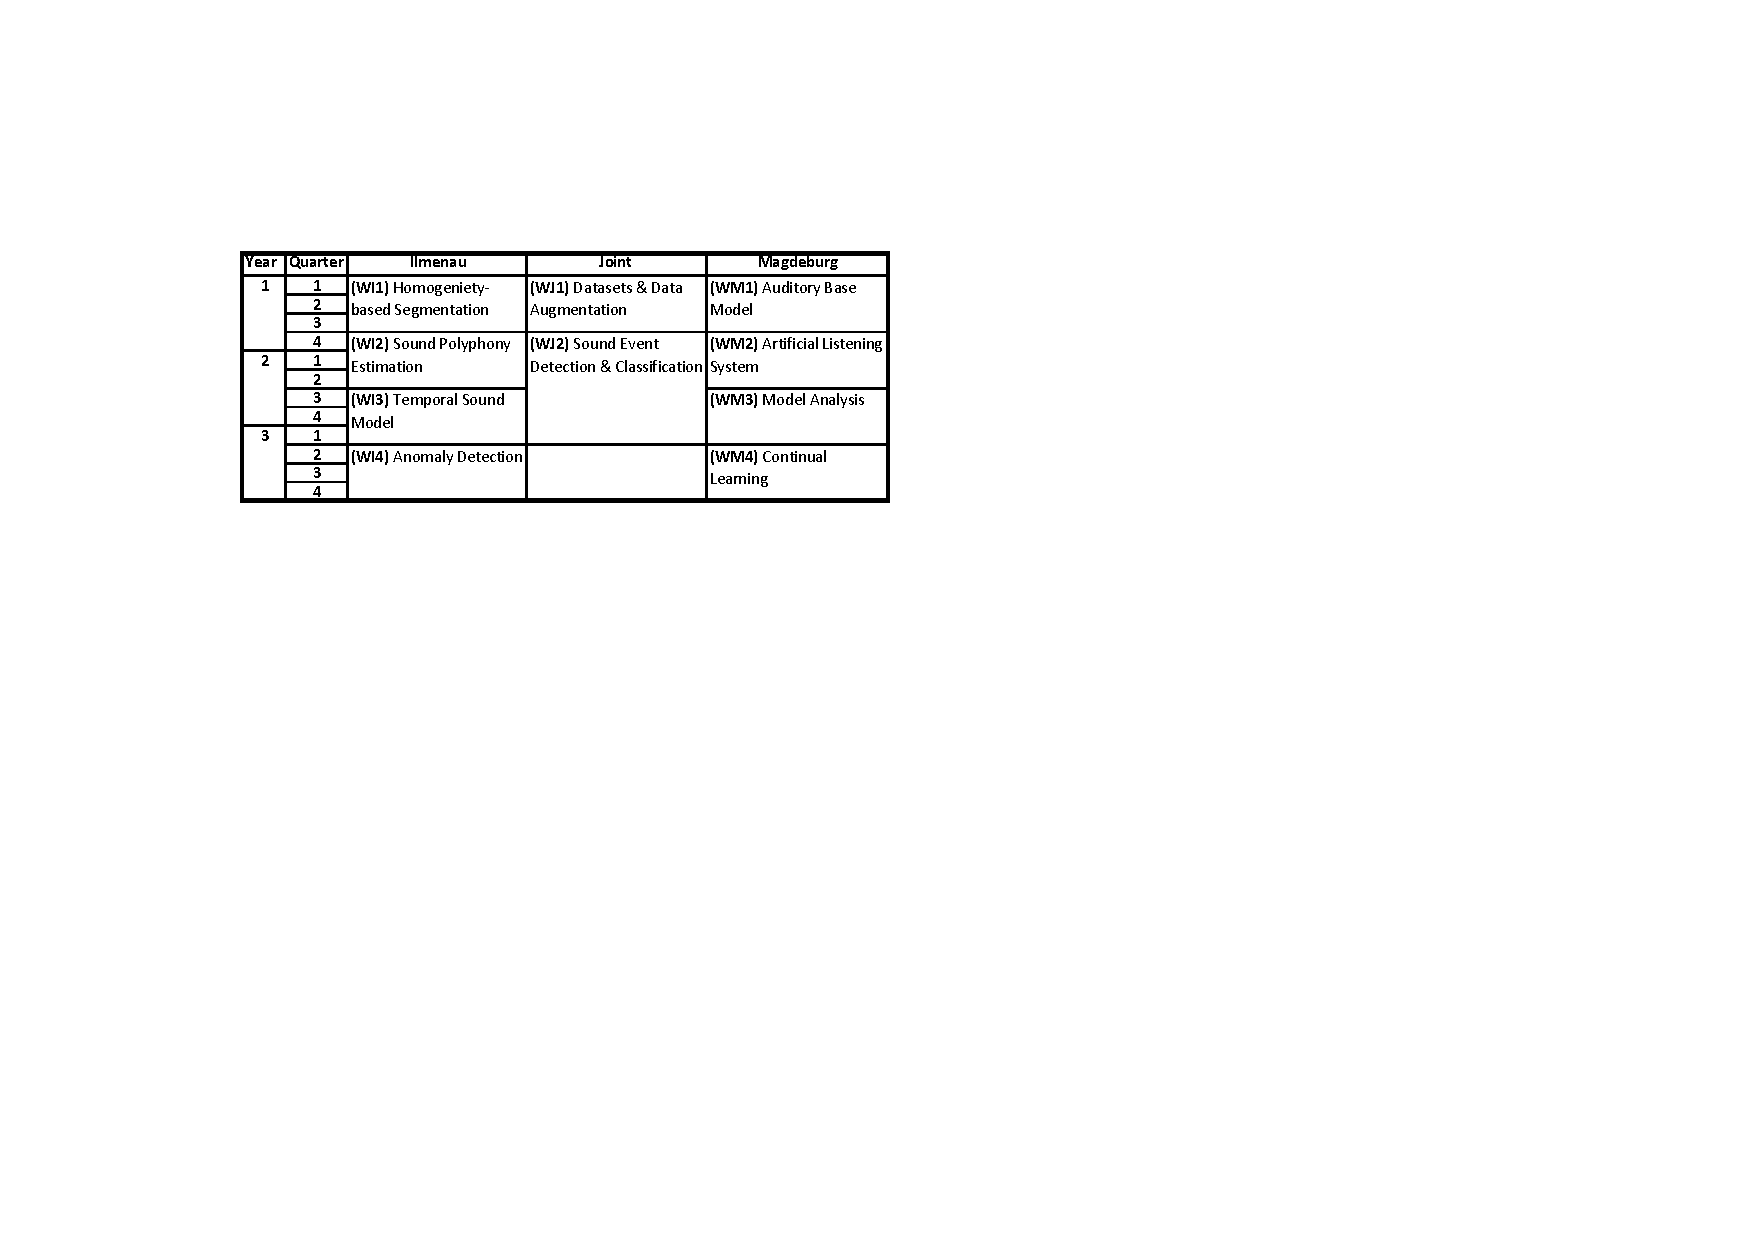
\includegraphics[width=.7\linewidth]{figures/wp_timetable.pdf}
 \label{fig:project_plan}
  \caption{Project structure illustrating both individual and joint work packages of the two research groups.}
  \end{figure}

In this section, eight individual work packages for the two research groups in Magdeburg (OVGU) and Ilmenau (IDMT) will be presented in sections \ref{sec:wi} and \ref{sec:wm} and two joint work packages will be introduced in section \ref{sec:wj}. Figure \ref{fig:project_plan} illustrates the overall project structure on a quarterly level.


% =======================================================================
\subsubsection{Work Packages Ilmenau}
\label{sec:wi}
% =======================================================================

% =======================================================================
\wpdef{I1}{Homogeniety-based Segmentation }
% =======================================================================

In this work package, we aim to subdivide long-term audio recordings into segments with homogeneous timbre characteristics. Such segments could for instance include stationary sounds such as rotating machines and passing trains or noise-like sounds such as rain and running water.
In Music Information Retrieval (MIR), similar attempts have been made to identify segments such as verse or chorus in music recordings \cite{Mueller:2015:MusicProcessing:BOOK}.
A common approach is to first identify points in time in which certain signal characteristics change (boundary detection). For that purpose, novelty functions are computed, which measure the local likelihood of a segment change. In a second step, segments are annotated based on their similarity relationship (segment labeling).

A first structure analysis approach that we aim to adapt to environmental sound recordings was presented by McCallum in \cite{McCallum:2019:Segmentation:ICASSP}. He trained a siamese network based on Constant-Q spectrogram snippets such that the similarity between two segments of a music recording is captured by the distance of their embedding representations.
Based on a self-similarity matrix of these embedding vectors, a novelty curve for boundary detection can be extracted.
An alternative approach to compute such a novelty curve based on the mismatch-first farthest-traversal principle was used by Zhao et al. in \cite{Zhao:2020:ActiveLearningSED:ARXIV}.
%Due to the large variety of timbre characteristics, we will focus instead on processing either spectrogram-like representations such as Mel spectrograms or audio signals using end-to-end modeling approaches.
McCallum uses a self-supervised training approach with the assumption that audio segments which are close in time are likely to sound similar.
In contrast, we aim to study further supervised training objectives based on existing sound class annotations and their similarity relationship based on sound taxonomies.
As one important aspect, we aim to study how the temporal overlap of multiple sounds will affect the novelty curves and the segmentation results.
As a second approach for structure analysis, we will study the recently proposed RepNet neural network architecture \cite{Dwibedi:2020:RepNet:CVPR}, which was proposed for class-agnostic detection of repetition in videos. We plan combine this approach with different audio embedding representations to reveal repetitive sound characteristics and structures in environmental audio recordings.
% 
% We aim to analyze multiple frequency bands simultaneously in order to being able to detect multiple repetitive sound events on multiple time-scales.

% TODO https://y-wang.weebly.com/uploads/1/2/1/9/121941993/wang_fewshotsed_icassp2020.pdf

% =======================================================================
\wpdef{I2}{Sound Polyphony Estimation}
% =======================================================================
The segmentation estimated in \wpref{I1}{WI1} describes the temporal structure of a recorded acoustic scene.
As a complementary view, we aim to estimate the number of simultaneously audible sounds (sound polyphony) within each segment to measure the sound density in a given acoustic scene. 
Related tasks such as ensemble size estimation \cite{Grollmisch:2019:EnsembleSize:CMMR}
and music polyphony estimation \cite{Kareer2018} were investigated in the field Music Information Retrieval (MIR).
%While pitched music instruments such as guitars or piano share at least a common harmonic overtone structure, environmental sounds cover a large variety of spectral characteristics.
To the best of our knowledge, polyphony estimation in environmental sound recognition is a previously unexplored task, which is particularly challenging due to the large variety of spectral sound characteristics.

In this work package, we plan to approach the polyphony estimation (PE) task by first performing a broad categorization of the segments, which were identified in \wpref{I1}{WI1}, into one or multiple general sound categories such as transient, harmonic, or noise-like sounds.
We want to use unsupervised clustering techniques to identify local patterns in spectrogram representations of the acoustic scene, which can indicate distinct sound events or components thereof. The number of such clusters will be used as indicator for the local sound polyphony.
Based on a global sound database, which will be collected in \wpref{J1}{WJ1}, and using the Scaper library\footnote{\url{https://github.com/justinsalamon/scaper}}, we will synthetically generate well-defined mixtures of different sound types and different degrees of polyphony, which will allow for training and evaluating different algorithmic approaches for PE.
% In particular, we plan to use the URBAN-SED\footnote{\url{http://urbansed.weebly.com/}} and DESED\footnote{\url{https://project.inria.fr/desed/}} datasets for evaluation within urban and domestic sound scenes.


% =======================================================================
\wpdef{I3}{Temporal Sound Model}
% =======================================================================

Most sound types appear multiple times within an long-term recording of a given acoustic scene. Examples for such sound types are bird singing, passing cars, or rotating machines in factories.
In this work package, we build upon the detected and classified sound events in \wpref{J2}{WJ2} and the overall structure determined in \wpref{I1}{WI1}.
In particular, we will try to detect typical appearance and repetition patterns of different sounds to get a better understanding on how particular sounds characterize acoustic scenes. Furthermore, we will study, whether certain sound types appear in a specific order. Such an order could for instance relate to a specific manufacturing process, which includes a fixed sequence of sub-tasks, or the general schedule on a construction site.

% =======================================================================
\wpdef{I4}{Anomaly Detection}
% =======================================================================

The goal of this work package is to detect previously unheard sounds (timbre novelty) as well as known sound events, which occur in unusual order or temporal frequency of repetition (temporal novelty).
For the former novelty type, we will quantify the timbre dissimilarity of a novel sound w.r.t.~sound events previously detected in \wpref{J2}{WJ2}.
Therefore, we will study the usefulness of different distance metrics in suitable embedding spaces. 
For the second novelty type, we use the temporal sound model of a given acoustic scene as developed in \wpref{I2}{WI2} to anticipate the order and repetition frequency of future sound events. 
As baseline systems, will re-implement several state-of-the-art AAD algorithms\footnote{Based on the results of the DCASE 2020 Challenge task 2 - Unsupervised Detection of Anomalous Sounds for Machine Condition Monitoring.}, which work on a frame-level instead of event-level signal representation. We plan to evaluate different strategies for anomaly detection in both urban and industrial sound scenarios.

% ==========================================

% =======================================================================
\subsubsection{Work Packages Magdeburg}
\label{sec:wm}
% =======================================================================

% =======================================================================
\wpdef{M1}{Auditory Base Model} %Modeling Atomic Sounds / Auditory Bases}%Domain Adaptation}
% =======================================================================
% -	Supervised and unsupervised DA methods\\
% -	Identification of semantic-preserving similarity measures to identify corresponding sounds in timbre feature space
%    -> maybe distance in latent space?
In this work package, we will train a generative model for atomic (i.e.,~short) sounds based on the DDSP approach originally proposed for monophonic music recordings \cite{engel2020ddsp}.
We will construct a VAE with a decoder that comprises several differentiable sound generators as well as additional differentiable signal processing modules that can modify the sound.
%These need to be adapted 
% comprises 
% \begin{itemize}
%     % differentiable version of Spectral Modeling Synthesis (SMS) Serra & Smith (1990)
%     \item an additive/sinusoidal synthesizer that synthesize audio with a bank of harmonic/arbitrary sinusoidal oscillators,
%     \item a noise filter synthesizer that synthesize audio by filtering white noise,
%     \item a wavetable synthesizer
% \end{itemize}
% as well as effect modules for reverb, exponential decay
The existing DDSP implementation follows a Harmonic-plus-Noise synthesis approach combining the output of an additive synthesizer (with multiple harmonic sinusoids) with a stream of filtered noise.
This suffices for modelling monophonic instruments but will be too limited within the context of this project as our prior experiments with speech and polyphonic music have already shown.
We will therefore investigate further extensions
such as basic physical modeling techniques 
or attack-decay-sustain-release (ADSR) envelope modeling.

In \cite{engel2020self}, DDSP has been successfully used to disentangle pitch from timbre, which is an important task in audio scene understanding.
We intend to extend this to further dimensions of sound quality / acoustic parameters.
Furthermore, DDSP allows to explicitly factorize the room acoustics (such as reverb) into a post-synthesis convolution step as shown in \cite{engel2020ddsp}.
This leads to an increased interpretability and allows to manipulate the room acoustics independently from the source sound. 
Such manipulation could be used for systematic data augmentation in \wpref{J1}{WJ1}.
Similarly, we will investigate the possibility to explicitly model microphone characteristics.

% TODO: Train with a large variety of short recordings (e.g. AudioSet)

% =======================================================================
\wpdef{M2}{Artificial Listening System} % Taxonomy Learning \& Hierarchical Classification}
% =======================================================================
% -	Unsupervised vs. semi-supervised taxonomy creation (data-driven vs. Knowledge-driven) based on sound similarity measures
% -	Flat vs. hierarchical classification
% - check Bones et al 2018 Frontiers in Psychology \cite{Bones:2018:SoundCategories:FIP} \\
% - multi-scale approach
%feedback mechanisms from cognitive brain networks that exploit prior knowledge (auditory memory) to guide attention to the target sound

%
\begin{figure}[h]
    \centering
    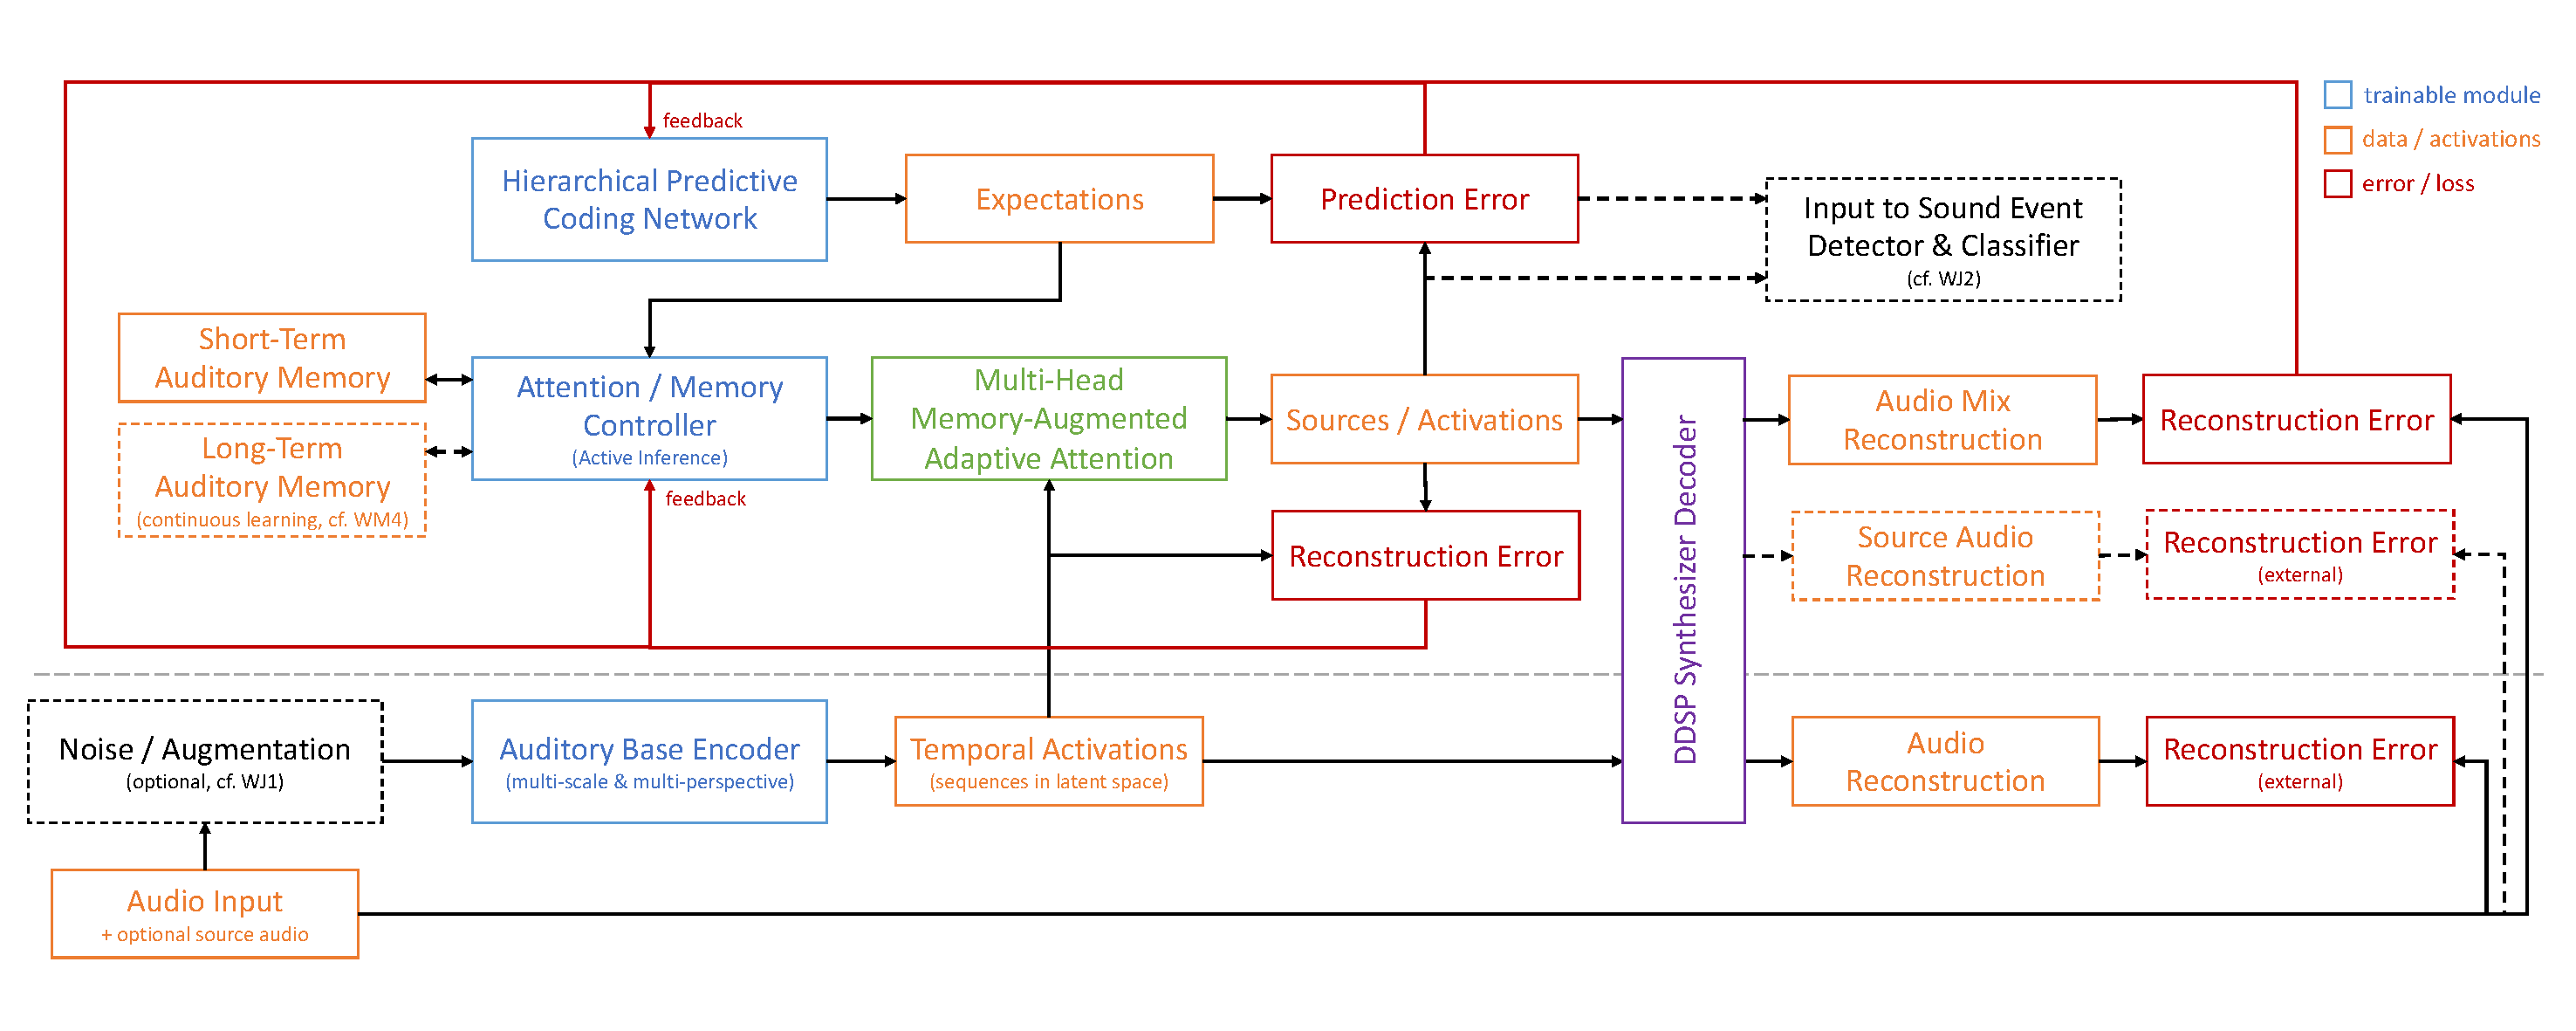
\includegraphics[width=\textwidth]{figures/artificial_listening_system.pdf}
    \vspace{-0.9cm}
    \caption{Overview of the artificial listening system (top) including the auditory base encoder (bottom)}
    \label{fig:artificial_listening_system}
\end{figure}
%
Using the auditory base encoder developed in \wpref{M1}{WM1} (shown in  \autoref{fig:artificial_listening_system}, bottom), temporal activations sequences can be computed for longer audio recordings.
These are then further processed by the artificial listening system developed in this work package.
The proposed high-level architecture and information flow is visualized in 
\autoref{fig:artificial_listening_system} (top).
Our approach is inspired by recent findings from cognitive and computational neuroscience on auditory perception modelling (e.g. \cite{chakrabarty2019gestalt,bellur2020taslp}).
% J. K. Bizley and Y. E. Cohen, “The what, where and how of auditory-object perception,” Nature Reviews Neu- roscience, vol. 14, no. 10, pp. 693–707, 2013.
The core of this architecture is an adaptive attention mechanism that is modulated by auditory memory and expectations obtained from a hierarchical predictive coding network.
Each attention head is driven by a prototypical sound event from memory (represented in the latent space) plus the top-down expectations about the respective temporal activity.
We hypothesize that this will significantly increase the robustness of detecting and separating sound events.
We will also experiment with a variable number of attention heads to adapt to the number of sources in the audio.
The result is similar to non-negative matrix factorization (NMF) with one matrix corresponding to the prototypical sound events in (short-term) memory and the other being the output of the attention mechanism.
In an offline processing setting, the memory could be initialized via NMF similar to the approach proposed in \cite{bellur2020taslp}.
There is also the option of multiple passes over the input audio for a better adaptation of attention mechanism -- similar to an experienced listener.
Alternatively, a general initialization could be learned in the training phase.
When processing a specific audio recording, the controller will adapt the memory content based on internal feedback signals that comprise the prediction error as well as the reconstruction error for the encoded audio and the raw signal.

The respective controller behaviour will be learned during the training phase together with the hierarchical predictive coding network. 
For both, we will investigate suitable architectures.
All other components shown in \autoref{fig:artificial_listening_system} (top) are input-dependent or not trainable (attention logic, loss functions, DDSP decoder).
For training, which is fully self-supervised, all internal and external errors can be used to provide gradients.
Optionally, the source audio reconstruction error can be evaluated if the actual source audio is available for supervised training.
As the order of the sources might differ, a best matching needs to be found first or the minimal error over all possible matching could be used.
For the audio reconstruction errors, a multi-scale spectral loss will be used as in \cite{engel2020ddsp}.

% doppelt:
% We will investigate suitable architectures for the controller and the predictive coding network.
% Here, we will benefit from the high degree of model interpretability, for instance:
% (1) The internal prediction and reconstruction error directly indicate potential problems.
% (2) Sources in memory can be sonified via the DDSP decoder
% (3) The ouput of the attention mechanism can be compared to ground-truth annotations for specific recordings.

% TODO: mention training sets? classification in another work package?

% =======================================================================
\wpdef{M3}{Model Analysis}% Model Validation}
% =======================================================================
% -	Defining \& implementing task-specific evaluation measures\\
% - novel evalation measures for polyphonic SED \cite{Bilen:2020:AEDEval:ARXIV} \\
% •	use XAI methods (LRP and alike) as sanity check, that relevant temporal-spectral components are recognized by the models (e.g. using synthetically created mixtures)

% for references: LRP on ISA \cite{grollmisch2020:isa_visualization} -> artificial unwanted bias added -> missbehaviour of model could be visualized

% Model analysis will be done at several levels.
%
First the auditory base encoder will be analyzed to explain how sounds are represented by the generative model.
In particular, this analysis will focus on understanding how the model encodes atomic sounds in the latent space.
We will investigate how the encoding connects to generated parameters for the synthesizer.
We expect the DDSP-VAE model to learn disentangled representations in a sense that different latent units represent different components of a sound.
Inspecting the representations in the DDSP model is possible by generating and listening to audio.
% which makes an auditory interpretation easy (in contrast to working with spectrograms). 
Typical end-to-end generative models do not always generate data that is easy to interpret. 
While unnatural images in computer vision can still be interpreted visually, unnatural sounds are much harder to interpret.
As DDSP only generates parameters for a synthesizer, the outputs are much more intuitive to acoustically interpret.

Explainable AI (XAI) methods from computer vision identify parts of the input feature representations that were important for the prediction.
For sound in form of spectrograms, this can give information about particular frequency bands and the time points which the model focuses on for the classification.
Especially the time points are interesting. 
We will use them to validate whether the Artificial Listening System developed in \wpref{M2}{WM2} predicts repeating sounds by attending to previous occurrences of this sound.
The importance of frequency bands is less intuitive to interpret.
Instead, we will adapt those XAI methods such that importance is not identified in the input space but in the representation space.
By generating sound using only the identified latent space positions, we can give audible explanations of predictions.

The predictive model developed in \wpref{M2}{WM2} will be analyzed regarding its predicted states in short and longer periods of time.
We will investigate the possible predictions for the next time step when given a sequence of observed audio.
This will be done by identifying the most likely next states and generating the corresponding sound for auditory inspection.
% Moreover, the most likely predictions will be traced back to the input by applying adapted methods from XAI.
Furthermore, we will investigate the long-term behaviour, whether there are base states which the model falls into, like noise, silence or endlessly repeating sounds.

To perform these analyses globally (i.e.~not only investigating single examples), we will compare homogeneous groups of inputs.
In our case, these are not given by labels of the examples.
Therefore, we are using the segments derived from \wpref{I1}{WI1} and the classified sound events derived in \wpref{J2}{WJ2}.
This way, we can specifically compare behaviour of the model for different types of inputs.

% =======================================================================
\wpdef{M4}{Continual Learning} % Continuous Learning}\\
% =======================================================================
% -	Evaluate continuous / active learning approaches to \\
% o	update the SED model by life-long learning of novel sound classes \\
% o	adapt the sound taxonomies (for hierarchical sound classification)
% few-shot learning

% ==========================================

We will investigate the capability of the artificial listening system to acquire and exploit a long-term auditory memory as indicated in \autoref{fig:artificial_listening_system} (left).
Such a memory could provide suitable candidates for initial short-term memory entries.
Through the design, this memory can easily be extended as the model is exposed to novel sounds during production without the need for re-training
because the trainable part of the model only comprises the control and prediction modules.
Thus, the model can quickly adapt to new sounds and  environments. 
%
To this end, we will extend the controller network to consider the additional memory for initialization and include a mechanism that decides when to extend the long-term memory.
%
For the identification of new event classes, an active learning strategy will be implemented which analyzes the internal error values of the artificial listening system as well as confidence values from the detector and classifier module.



% =======================================================================
\subsubsection{Joint Work Packages}
\label{sec:wj}
% =======================================================================

% =======================================================================
\wpdef{J1}{Datasets \& Data Augmentation}\label{WJ1}
% =======================================================================
Sound event detection datasets contain either strongly-labeled or weakly-labeled annotations. While the former provide precise information about the starting time and duration of each annotated sound event, such annotations require a high annotation effort. Weakly-labeled annotations on the other hand are cheap to create but only provide information about the presence of certain sound events in an audio recording without their precise time of occurrence. 
%If a sound is only audible in a short part of a recording, such annotation introduces severe label noise in the training of a classifier. 
%As a possible solution, strong labels can be simulated by repeating weak labels \cite{Adavanne:2017:AEDWeaklyLabels:DCASE} to create frame-level annotations. Alternatively, a temporal pooling step can be integrated into AED algorithms to aggregate frame-level predictions to file-level tags, which can be compared with weak labels during training.
As alternatives strongly labeled data, SED algorithms can be trained using sequentially labeled data, which informs about the temporal order but not the exact occurrence times of audio events \cite{Hou:2019:SoundEvent:ICASSP} or using point-wise labeled data \cite{Kim:2019:PointWise:WASPAA} where each sound is only annotated in on frame.

In this work package, we will compile and merge at least 15 different publicly available SED datasets to a global sound database. 
Here, we will unify different annotations schemes (weak vs. strong labels, single-label vs. multi-label, etc.) and audio formats (different sample rates, number of channels).
Also, we will investigate, whether hierarchical relationships between sound events can be defined, which could be exploited later for SED in  \wpref{J2}{WJ2}.
In addition to the existing datasets, we plan to conduct several audio field recording in specific environments such as industrial fabrication lines, nature locations, and urban scenes and annotate them w.r.t. occurring sound events.

As another basis for the experiments in \wpref{J2}{WJ2}, we will intregrate several state-of-the-art data augmentation methods such as SpecAugment and mixup into the SED training pipeline in \wpref{J2}{WJ2}. As one specific approach, we plan to measure the impulse responses of several microphone types in the Fraunhofer IDMT facilities to be able to simulate different microphone characteristics during the model training to improve the robustness of the SED models.


% =======================================================================
\wpdef{J2}{Sound Event Detection}
% =======================================================================

This joint work package bundles all activities towards developing a general-purpose SED model.
Based on the global sound database, which is assembled in \wpref{J1}{WJ1}, we will first define multiple experimental settings of increasing complexity. Each setting will include a subset of the available sound classes as well as a specific strategy on how to split the data into training, validation, and test sets for the model training and evaluation. Such settings will be aligned to targeted sound categories such domestic sounds, industrial sounds, or urban sounds. 

The main focus then will be on a comparative evaluation of different modeling pipelines, which involve algorithms for audio pre-processing, feature extraction, and data modeling.
Concerning the audio signal representation, we will compare both end-to-end modeling approaches, which take raw audio samples as model input, with spectrogram-based approaches, where two-dimensional representations such as mel-spectrograms, or STFT are processed. Specialized pre-processing methods such as Per-Channel Energy Normalization (PCEN) \cite{Lostanlen:2018:PCEN:SPL} will be tested to suppress stationary noise components and better focus on foreground sound events.
Given the latest scientific publications in the field of SED, we will assemble and re-implement the most promising deep neural network architectures covering CNN, CRNN, and attention-based models \cite{Zhang:2020:FrameLevelAttention:ARXIV} as baseline systems.
Special focus will be put on strategies to cope with the high variance of sound durations
using for instance multi-scale modeling approaches such as AdaMD \cite{Ding:2020:AdaMD:IEEE_TASLP} and memory-controlled sequential self attention \cite{Pankajakshan:2020:MSSSelfAttention:ARXIV}. 

Using the data augmentation methods implemented in \wpref{J1}{WJ1} and methods for domain adaptation \cite{Drossos:2019:DomainAdaptation:WASPAA}, we aim to improve the robustness and generalizability of the developed SED model towards previously unheard audio recording conditions. Possible strategies involve context-adaptive neural networks (CA-NN) \cite{Lostanlen:2019:EventDetection:PLOS}, which involve the modeling of the background noise into the SED task.
%One additional research direction, which we plan to investigate in this joint work package, is to test unsupervised and self-supervised learning strategies to benefit from additional data sources without any sound event description.

% We will furthermore test two attention based strategies. Ding and He  propose the adaptive multi-scale AED (AdaMD) approach where an audio signal is processed using an autoencoder-like network, which first compresses the signal into a lower-dimensional representation before restoring it. 
% Intermediate representations from the decoder, which correspond to different time scales, are  modeled using separate bi-directional recurrent layers before the outputs are combined.
% A frame-level attention mechanism, which is integrated both in the front-end CNN layers as well as the back-end RNN layers, was proposed by Zhang et al  to enforce sound classification models on semantically relevant and non-silent frames.

% TODO integrate
% As one possible solution, multi-scale approaches such as the AdaMD algorithm \cite{Ding:2020:AdaMD:IEEE_TASLP} use multiple time resolutions for classification simultaneously.

% TODO integrate 
% The attention width of such models often needs to be constraint to avoid that they overly focus on irrelevant correlations between successive spectrogram frames. Memory-controlled sequential self attention \cite{Pankajakshan:2020:MSSSelfAttention:ARXIV} allows to simultaneously use and combine multiple attention spans using a multi-head attention structure. This way, AED systems can analyze multiple time resolutions simultaneously and better recognize sound events of different lengths.

% =======================================================================
\renewcommand{\refname}{Bibliography Concerning the State of the Art, the Research Objectives, and the Work Programme}
\section{Bibliography Concerning the State of the Art, the Research Objectives, and the Work Programme}
\begingroup
\renewcommand{\section}[2]{}%
\bibliography{refs_final_compressed}
\endgroup
% =======================================================================

\section{Relevance of sex, gender and/or diversity}
The combined research team at the OVGU Artificial Intelligence Lab and the Fraunhofer Institute for Digital Media Technology (IDMT) spans several dimensions of diversity such as gender, cultural background, and research disciplines -- including computer science, bioinformatics, cognitive science, medical systems engineering, electrical engineering, and acoustics.
The resulting inter-disciplinary perspective is a core element of this project.


\section{Supplementary information on the research context}

\subsection{Ethical and/or legal aspects of the project}

As a basis for the planned field recordings in \wpref{J1}{WJ1}, we will obtain all relevant permits from local authorities. Furthermore, we will inform the public about ongoing audio recordings.
To meet data protection requirements, unintentionally recorded speech is cut out or obfuscated before audio recordings and the corresponding annotations are published.
Here, we can rely on existing expertise from the Media Distribution and Security group at Fraunhofer IDMT.

\subsubsection{Descriptions of proposed investigations involving experiments on humans or human materials}

Not applicable.
\vspace{-.3cm}

\subsubsection{Descriptions of proposed investigations involving experiments on animal}

Not applicable.
\vspace{-.3cm}

\subsubsection{Descriptions of projects involving genetic resources (or associated traditional knowledge) from a foreign country}

Not applicable.
\vspace{-.3cm}

\subsubsection{Descriptions of investigations involving dual use research of concern, foreign trade regulations}

Not applicable.
\vspace{-.3cm}


% =======================================================================
\subsection{Data Handling}
% =======================================================================

In order to foster reproducibility in science, we will mainly use data resources which are publicly available.
In return, we will publish all novel audio field recordings made in \wpref{J1}{WJ1} including SED annotations to the scientific community on a suitable project website to stimulate further research.
We also plan to regularly demonstrate current research results on a designated project website. This will include software demonstrators, suitable code libraries, as well as sound examples.



% =======================================================================
\subsection{Other Information}
% Please use this section for any additional information you feel is relevant which has not been provided elsewhere.
% =======================================================================
Not applicable.
\vspace{-.3cm}
% =======================================================================
\section{People/collaborations/funding}
% =======================================================================

% =======================================================================
\subsection{Employment status information}
%  For each applicant, state the last name, first name, and employment status (including duration of contract and funding body, if on a fixed-term contract).
% =======================================================================

Stober, Sebastian, University Professor (Otto von Guericke University Magdeburg, W2, tenure) \\
Abeßer, Jakob, Senior Scientist (Fraunhofer IDMT, TVÖD 13, 100 \%, unbefristet)

% =======================================================================
\subsection{First-time proposal data}
Not applicable.
% =======================================================================

% =======================================================================
\subsection{Composition of the project group}
% List only those individuals who will work on the project but will not be paid out of the project funds. State each person’s name, academic title, employment status, and type of funding.
% =======================================================================

\paragraph{Research Group in Ilmenau}
% TODO: explain who will contribute with how many percent and with which topics / expertises
% =======================================================================
The working group in \textbf{Ilmenau (Fraunhofer IDMT)} comprises of the following research staff:

\begin{table}[h!]
\begin{tabular}{lll}
 Jakob Abeßer, Dr-Ing. & Senior Scientist   \\
 Sascha Grollmisch & PhD student / Wissenschaftlicher Mitarbeiter \\
 David-Scott Johnson, Dr. & Post-Doc / Wissenschaftlicher Mitarbeiter \\
Hanna Lukashevich & Head of Semantic Music Technologies Group \\
Christon Ragavan Nadar & PhD student \\
Stylianos Ioannis Mimilakis  & PhD student \\
Michael Taenzer  & PhD student \\
\end{tabular}
\end{table}

The following people will contribute to the SoReLUA-project: the funded staff member (100 \% for 36 months), Jakob Abeßer (10 \%, supervision, organization, project work), Sascha Grollmisch and David-Scott Johnson (15 \%, project work, synergies to their work on sound event detection and industrial sound analysis), Hanna Lukashevich (10 \%, synergies to her work on machine learning for music information retrieval), as well as Christon Ragavan Nadar, Stylianos Ioannis Mimilakis, and Michael Taenzer (5 \%, project work, synergies to their work on music and audio classification). Furthermore, the technical infrastructure of the Fraunhofer IDMT can be used.

\paragraph{Research Group in Magdeburg}
% TODO: explain who will contribute with how many percent and with which topics / expertises
% =======================================================================
The working group in \textbf{Magdeburg (OVGU)} comprises of the following research staff: 
\begin{table}[h!]
\begin{tabular}{ll}
Sebastian Stober, Prof.~Dr.-Ing.     &  Head of the research group \\
Andreas Krug        & PhD student / Wissenschaftlicher Mitarbeiter \\
Jens Johannsmeier   & PhD student / Wissenschaftlicher Mitarbeiter \\
André Ofner         & PhD student / Wissenschaftlicher Mitarbeiter \\
Jan-Ole Perschewski & PhD student / Wissenschaftlicher Mitarbeiter \\
Maral Ebrahimzadeh  & PhD student / Wissenschaftliche Mitarbeiterin \\
Johann Schmidt      & PhD student / Wissenschaftlicher Mitarbeiter \\
Suhita Ghosh        & PhD student / Stipendiatin \\
\end{tabular}
\end{table}

The following people will contribute to the project besides the dedicated funded staff member: 
Sebastian Stober (10 \%, supervision, organization, project work),
Andreas Krug (10 \%, project work, synergies to his work on introspection techniques),
Jens Johannsmeier (10 \%, project work, synergies to his work on generative models -- especially VAEs),
André Ofner (10 \%, project work, synergies to his work on predictive coding),
Jan-Ole Perschewski and Maral Ebrahimzadeh (10 \%, project work, synergies to their work on explainable AI and introspection techniques within the CogXAI project).
Furthermore, the technical staff will provide support for the GPU-compute and data storage infrastructure to be used within the project.

% =======================================================================
\subsection{Researchers in Germany with whom you have agreed to cooperate on this project}
% =======================================================================
Prof. Dr. Meinard Müller (Audiolabs Erlangen) \\ % approved
Prof. Dr. Gerald Schuller (TU Ilmenau) \\ % approved
Senior Prof. Dr. Karlheinz Brandenburg (TU Ilmenau) \\ % approved

% =======================================================================
\subsection{Researchers abroad with whom you have agreed to cooperate on this project}
% =======================================================================
% 

Dr. Emmanouil Benetos (Machine Listening Lab, Queen Mary University, London, UK) \\ % approved
Prof. Tuomas Virtanen (Audio Research Group, Uni Tampere, Finland)\\ % approved
Dr. Konstantinos Drossos (Audio Research Group, Uni Tampere, Finland) \\ % approved
Prof. Gael Richard (Télécom ParisTech, Paris, France)\\ % approved  
Prof. Mark Plumbley (Surrey, UK) % approved


% =======================================================================
\subsection{Researchers with whom you have collaborated scientifically within the past three years}
% =======================================================================
Prof. Dr. Meinard Müller (Audiolabs Erlangen) \\ 
Dr. Christof Weiß (Audiolabs Erlangen) \\
Dr. Stefan Balke (pmOne Group) \\
Dr. Estefanía Cano (AudioSourceRe) \\
Prof. Martin Pfleiderer (HfM Weimar) \\
Dr. Klaus Frieler (HfM Weimar) \\
Prof. Dr. Christian Beste (TU Dresden)\\
Prof. Dr. Carsten Beta (University of Potsdam)\\
David A.~Bridwell (Mind Research Network, Albuquerque, USA)\\
Vince D.~Calhoun, Ph.D. (Center for Translational Research in Neuroimaging and Data Science, USA)\\
James F.~Cavanagh, Ph.D. (University of New Mexico, Albuquerque, USA)\\
Anne G.~E.~Collins, Ph.D. (UC Berkeley, USA)\\
Prof. Dr. Emrah Düzel (German Center for Neurodegenerative Diseases (DZNE), Magdeburg)\\
Prof. Dr. Marc Dewey (Charité, Berlin)\\
Michael D.~Nunez, Ph.D. (UC Irvine, USU)\\
Prof. Dr. Andreas Nürnberger (Otto von Guericke University Magdeburg)\\
Jun.-Prof. Dr. Kerstin Ritter (Charité, Berlin)\\
Prof. Dr. Harald Sack (FIZ Karlsruhe) \\
Ramesh Srinivasan, Ph.D. (UC Irvine, USA)\\
Prof. Dr. Manfred Stede (University of Potsdam)\\
Prof. Dr. Henrik Walter (Charité, Berlin)\\
%
%This information will help avoid potential conflicts of interest.

% =======================================================================
\subsection{Project-relevant cooperation with commercial enterprises}
% =======================================================================
Not applicable.
\vspace{-.3cm}
% If applicable, please note the EU guidelines on state aid or contact your research institution in this regard.

% =======================================================================
\subsection{Project-relevant participation in commercial enterprises}
% =======================================================================
Not applicable.
\vspace{-.3cm}
% Information on connections between the project and the production branch of the enterprise

% =======================================================================
\subsection{Scientific equipment}
\label{existing_equipment}
% =======================================================================
% List larger instruments that will be available to you for the project. These may include large computer facilities if computing capacity will be needed. 

Both the technical infrastructures of Fraunhofer IDMT and the OVGU will be available for the project staff during the applied project duration.
Fraunhofer IDMT's headquarter is located on the campus of the Ilmenau University of Technology (IUT) in a modern building with labs and offices and provides significant R\&D infrastructure regarding servers, GPUs, and available datasets especially regarding audio research. Fraunhofer IDMT also has access to relevant research facilities at the IUT.
Since founding the Artificial Intelligence Lab at the OVGU in October 2018, the group has been building a dedicated compute and storage infrastructure for teaching deep learning and running deep learning experiments.
This cluster is a shared effort of the Faculty of Computer Science at OVGU and comprises a central storage server (> 100 TB with full mirror redundancy) and currently nine GPU-compute nodes with 4 or 8 Nvidia graphic cards (GPUs) connected via a 100G Ethernet network.
Furthermore, the Artificial Intelligence Lab has dedicated servers for securely storing datasets and archiving trained models together with their training logs for reproducibility of the experiments.
The available compute nodes are all tied to specific projects within different research groups and to teaching activities respectively
and as the group continues to train more young researches in deep learning techniques, a further increasing demand for GPU-compute capacity is anticipated.
We therefore apply for funding of an additional GPU compute resources dedicated exclusively to this project (cf.~\ref{big_equipment}).
All other resources of Artificial Intelligence Lab the will be made available to the project.



% =======================================================================
\subsection{Other submissions}
% =======================================================================
% List any funding proposals for this project and/or major submitted. If we make such proposal, we will immediately inform the German research foundation.
Not applicable.
\vspace{-.3cm}
% =======================================================================
\section{Requested Modules/Funds}
% =======================================================================
% Explain each item for each applicant (stating last name, first name).

% =======================================================================
\subsection{Basic Module}
% =======================================================================

% =======================================================================
\subsubsection{Funding for Staff}
% =======================================================================

\paragraph{Scientific staff (full position, TVÖD 13, 36 months, Ilmenau).} 

The staff member takes over the work in Ilmenau throughout the total duration of the project. 
She/he needs to have excellent qualifications in the areas of Audio Signal Processing and Machine Learning with a focus on Deep Learning. Furthermore, very good programming skills in Python including prior knowledge of common machine learning libraries such as scikit-learn, keras, tensorflow, or pytorch are required.

\paragraph{Scientific staff (full position, TV-L 13, 36 months, Magdeburg).}

The staff member takes over the work in Magdeburg throughout the total duration of the project. 
She/he needs to have excellent qualifications in the areas of Deep Learning and Digital Signal Processing. 
Furthermore, very good programming skills in Python including prior knowledge in the deep learning framework tensorflow or pytorch is required.


\paragraph{Four student assistants (à 36 months à 30h/month, Ilmenau and Magdeburg)}

In the SoReLUA project, we aim to introduce motivated students to machine listening research problems at an early stage of their studies.
Therefore, we ask for four student assistants (two in Ilmenau and two in Magdeburg) to support the staff members. The students are required to have excellent programming skills in Python as well as a solid knowledge in the fields of audio processing and machine learning and will take over the following tasks.
First, signal processing and machine learning algorithms from the scientific literature need to be re-implemented, adapted, and evaluated as part of the respective SoReLUA work packages. 
Second, annotations of existing SED datasets need to be checked and maintained. 
Third, audio field recordings will be performed and annotated in different recording locations ranging from industrial factories, urban environments, as well as places in nature.
Finally, web-based interfaces and demonstrators are to be implemented to support the project dissimination.


% =======================================================================
\subsubsection{Direct Project Costs}
% =======================================================================

% =======================================================================
\paragraph{Equipment up to EUR 10,000, Software and Consumables}
% =======================================================================
In order to enable mobile field recordings in specific locations such as nature environments, urban locations, as well as industry settings, we plan to purchase two portable audio recording devices combined accessories (bag, memory card, windshield).
% https://www.thomann.de/de/sony_pcm_d100_bundle.htm
In order to store datasets, models and training logs for reproducibility of the experiments, the existing archive server in Magdeburg (cf.~\ref{existing_equipment}) will be extended by additional hard drives (in a ZFS raidz1 setup).
The following expenses are required:
% https://www.heise.de/preisvergleich/western-digital-ultrastar-dc-hc550-18tb-wuh721818al5204-0f38353-a2322034.html?hloc=de

\begin{table}[h!]
\centering
\begin{tabular}{lrr}
 Sony PCM-D100 Audio Recorder + Accessories
 & 2 $\times$ 640 EUR & 1,280 EUR  \\
 14TB HDD Western Digital Ultrastar DC HC530 & 3 $\times$ 433 EUR & 1,299 EUR  \\
 \hline
 \textbf{Total} &  &   \textbf{2,579 EUR}  \\
\end{tabular}
\end{table}

% instrumentation previously submitted to a third party

% No other application for funding of this project has been 

% =======================================================================
\paragraph{Travel Expenses}
% =======================================================================

All research results shall be published and presented in major international conferences (ICASSP, WASPAA, DCASE, NeurIPS, ICMR, ICML, etc.).
We expect each of the two staff members to visit two international conferences (with an estimated
cost of 2,000 EUR per conference comprising overseas 
ight, hotel, and registration fee). In addition, we expect  several smaller national conferences, workshops and bi-annual project meetings. In total, we expect costs of EUR 5,000 per year and per staff member, which leads to travel costs of \textbf{30,000 EUR} over three years.

% =======================================================================
\paragraph{Visiting Researchers}
% excluding Mercator fellow
% =======================================================================
We would like to invite at least one guest scientist per year per project partner for a guest talk (estimated at 500 EUR per visit) resulting in a total amount of 
3,000 EUR.

% =======================================================================
\paragraph{Expenses for Laboratory Animals}
% =======================================================================
Not applicable. 
% =======================================================================
\paragraph{Other Costs}
% =======================================================================
Not applicable. 
% =======================================================================
\paragraph{Project-Related Publication Expenses}
% =======================================================================
We apply for publication costs in the amount of \textbf{2,250 EUR} over the three year project duration, which we plan to use primarily for journal publications in renowned journals such as the IEEE/ACM Transactions on Audio, Speech, and Language Processing, the Journal of the Acoustical Society of America, the IEEE Signal Processing Magazine, or the Journal of Machine Learning Research.

% =======================================================================
\subsubsection{Instrumentation}
% =======================================================================

% =======================================================================
\paragraph{Equipment exceeding EUR 10,000}
\label{big_equipment}
% =======================================================================
For the project, dedicated GPU-compute resource are required both in Ilmenau and Magdeburg (cf.~\ref{existing_equipment}).
Based on our experience from earlier projects, a node with 8 high-end consumer GPUs will perfectly support one PhD student and the supporting student research assistants.
In the past, we have made very positive experience with a two-height-units server platform with a configuration as found in the appended offer. 
Very recently, a new generation of high-end consumer GPUs suitable for the deep learning experiments in this projects has been released by Nvidia -- the Geforce 3090.
However, as this new model came with several design changes, suppliers and server manufacturers are still in the process adapting and testing their platforms.
Therefore, we have not yet been able to obtain a suitable offer for respective GPU nodes with the new models.
We estimate a price increase by about 500 EUR per GPU resulting in a price of approximately 24,000 EUR per server.

\begin{table}[h!]
\centering
\begin{tabular}{lrr}
 GPU Compute Server (Ilmenau)
 & 1 $\times$ 24,000 EUR & 24,000 EUR  \\
 GPU Compute Server (Magdeburg)
 & 1 $\times$ 24,000 EUR & 24,000 EUR  \\
 \hline
 \textbf{Total} &  &   \textbf{48,000 EUR}  \\
\end{tabular}
\end{table}

% =======================================================================
\paragraph{Major Instrumentation EUR 50,000}
% =======================================================================
Not applicable. 

% =======================================================================
%\subsection{Module Temporary Position for Principal Investigator}
% =======================================================================

% =======================================================================
%\subsection{Module Replacement Funding}
% =======================================================================

% =======================================================================
%\subsection{Module Temporary Clinician Substitute}
% =======================================================================

% =======================================================================
%\subsection{Module Mercator Fellows}
% =======================================================================

% =======================================================================
\subsection{Module Project-Specific Workshops}
% =======================================================================
% https://www.dfg.de/formulare/52_01/52_01_en.pdf

A two-day workshop with all cooperating scientists, external scientists, as well as interested students will be held in Erfurt in spring 2022 to present and discuss the project outcomes and to derive further research questions. The main goal of this workshop is to strengthen the national machine listening research community and to stimulate corporations with international research institutions.  
The following expenses are required:

\begin{table}[h!]
\centering
\begin{tabular}{lrrr}
 Travel costs foreign countries & 4 $\times$ & 500 EUR & 2,000 EUR  \\
  Domestic travel expenses & 4 $\times$ & 100 EUR & 400 EUR  \\
 Two overnight stays & 8 $\times$ & 150 EUR & 1,200 EUR  \\
 \hline
 \textbf{Total} &  &  &  \textbf{3,600 EUR}  \\
\end{tabular}
\end{table}


%\todo{organisa-tional expenses}
% =======================================================================
\subsection{Module Public Relations Funding}
% =======================================================================

% https://www.dfg.de/formulare/52_07/52_07_en.pdf

%State and justify the requested funding amount. Discuss the following aspects, which will be considered in the review of the proposal: ƒPublic-relations objective and target-group description ƒRelationship of planned activities to the project/topic ƒInvolvement of the institution’s public relations department 

In order to make the methods and findings of this project accessible to a wider range of young researches, we plan to organize a three-day summerschool for 10 PhD students at the Fraunhofer IDMT facilities in the final year of the project (summer 2023).
In this summer school, different lectures on deep learning and machine listening topics will be held. Furthermore, the students will participate in practical coding seminars, in which acquired basic knowledge is to be applied in practical application projects. Possible topics will include the miniaturization and deployment of machine listening algorithms onto embedded sensor systems, explainable AI techniques, automatic traffic monitoring, and sound recognition in industrial end-of-line testing scenarios.
During the organization of the workshop, the Fraunhofer IDMT public relation department will assist us with their expertise.
Furthermore, we will actively involve the student assistants in the organization process.
The following expenses are required:

\begin{table}[h!]
\centering
\begin{tabular}{lrrr}
  Domestic travel expenses  & 10 $\times$ 2  $\times$ & 100 EUR & 2,000 EUR  \\
 Two overnight stays & 10 $\times$ 2  $\times$ & 150 EUR & 3,000 EUR  \\
 Catering costs & 10  $\times$ & 120 EUR & 1,200 EUR  \\
 \hline
 \textbf{Total} &  &  &  \textbf{6,200 EUR}  \\
\end{tabular}
\end{table}



\end{document}
